\begin{answer}
\begin{figure}
  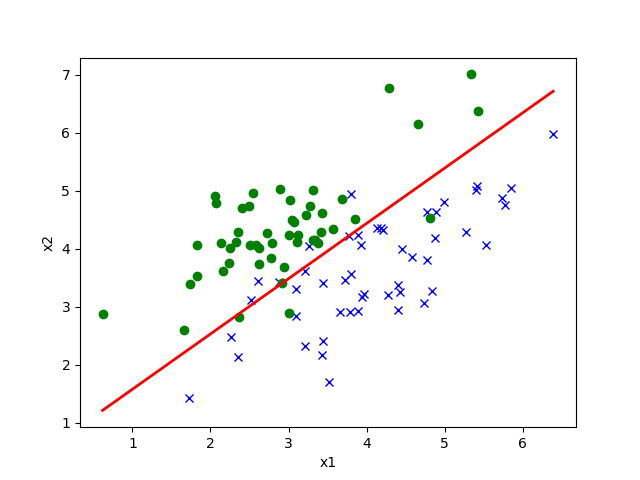
\includegraphics[width=\linewidth]{../src/output/p01b_pred_2_eval.png}
  \caption{Dateset 2 prediction on VALIDATION set using LogisticRegression}
  \label{fig:Dateset 2 prediction on VALIDATION set using LogisticRegression}
\end{figure}\\
\begin{figure}
  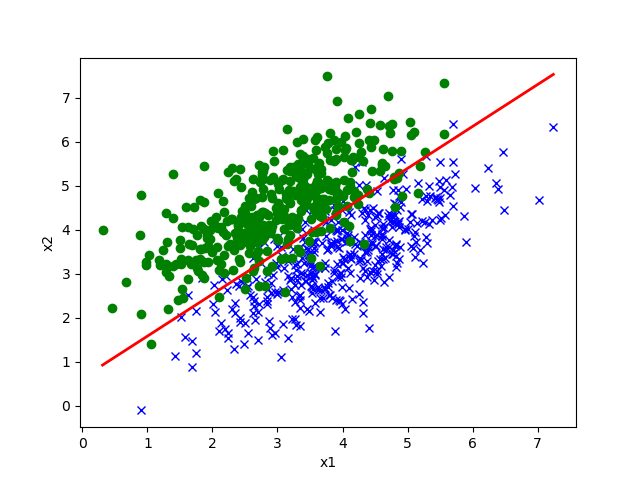
\includegraphics[width=\linewidth]{../src/output/p01b_pred_2_train.png}
  \caption{Dateset 2 prediction on TRAIN set using LogisticRegression}
  \label{fig:Dateset 2 prediction on TRAIN set using LogisticRegression}
\end{figure}\\
\begin{figure}
  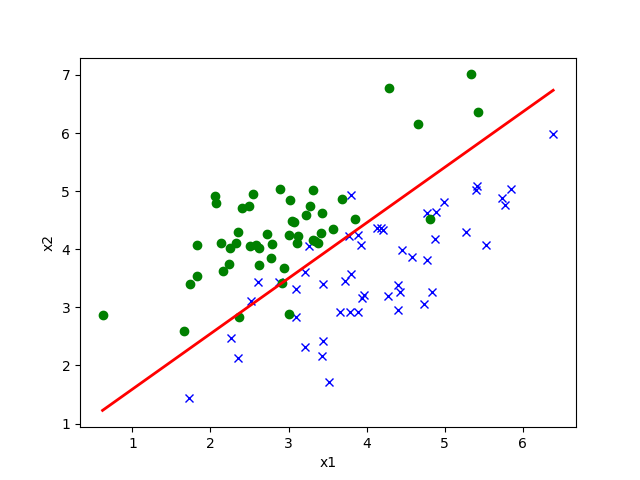
\includegraphics[width=\linewidth]{../src/output/p01e_pred_2_eval.png}
  \caption{Dateset 2 prediction on VALIDATION set using GDA}
  \label{fig:Dateset 2 prediction on VALIDATION set using GDA}
\end{figure}\\
\begin{figure}
  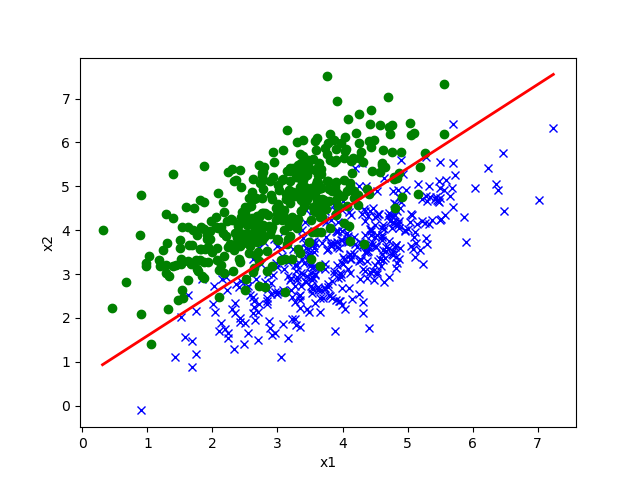
\includegraphics[width=\linewidth]{../src/output/p01e_pred_2_train.png}
  \caption{Dateset 2 prediction on TRAIN set using GDA}
  \label{fig:Dateset 2 prediction on TRAIN set using GDA}
\end{figure}\\
GDA does worse on the first dataset. This is the case because we have some points that are outliers that are skewing the calculations of $\mu_0, \mu_1$ and $\sigma$. 
\end{answer}
